\documentclass[12pt]{article}
%--------------------   start of the 'preamble'
%
\usepackage{graphicx,amssymb,amstext,amsmath,color}
\usepackage[margin=2cm]{geometry}
\usepackage{abstract}
\usepackage{setspace}
\usepackage[footnotesize,bf]{caption}

% TABLE
\usepackage{multicol,hhline,colortbl,multirow}
\usepackage{braket}
\usepackage{siunitx}
\usepackage{hyperref}
\usepackage{authblk}
\usepackage{siunitx}
\usepackage{mathrsfs}
%%\usepackage[sort&compress]{natbib}
%%\bibpunct{(}{)}{,}{a}{, }{;}
%
\usepackage[sort&compress]{natbib}
\bibpunct{[}{]}{,}{s}{}{;}


\definecolor{gray}{gray}{0.8}
\def\mobunits{\square\centi\meter\per\volt\per\second}
\def\gcm{\gram\per\cubic\centi\meter}
\def\ccg{\cellcolor{gray}}

\renewcommand{\labelitemii}{$\circ$}
\renewcommand{\bibname}{References}


\title{MorphCT Results - Device Simulations}
\author{Matthew Jones}
\date{\today}

\begin{document}
\maketitle


\section{Test System}

NOTE: We still don't have a real device morphology to work with, so I've bodged one together from the data we already have.
It will not suffice for publication, but I'm hoping it will allow me to get all the moving parts in place before we set the code loose on a physical system

\begin{figure}[h!]\centering
	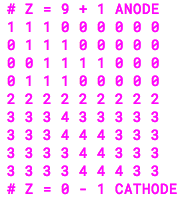
\includegraphics[width=0.3\textwidth]{Figures/device.png}
    \caption{A single slice of the test device used to write and configure the device-scale KMC code}
	\label{fig:device}
\end{figure}

\begin{center}
\begin{tabular}{| c | c | c | c |}
\hline
\rule{0pt}{2.5ex} 
\multirow{2}{*}{\textbf{ID}}&\multirow{2}{*}{\textbf{Simulation Name}}&\multirow{2}{*}{\textbf{XML Name}}&\textbf{$l_{x,y,z}$}\\
                            &&&(\SI{}{\AA})\\
\hhline{|====|}
\rule{0pt}{2.5ex}\textbf{\ccg0}&\ccg orderedP3HT&\ccg p1-L15-f0.0-P0.1-T1.5-e0.5&\ccg 85.19\\
\textbf{1}&disorderedP3HT&shrunkp1-L15-f0.0-P0.1-T2.0-e0.5&85.19\\
\textbf{\ccg2}&\ccg interfaceP3HTC60&\ccg p1-L15-f0.3-P0.1-T1.5-e0.1&\ccg 96.23\\
\textbf{3}&disorderedPCBM&pcbm-0.5-P0.5-300-T3.0\_AA&65.69\\
\textbf{\ccg4}&\ccg orderedPCBM&\ccg pcbm-0.5-P1.5-200-T5.0\_AA&\ccg 57.53\\
\hhline{----}
\end{tabular}\label{table:cells}
\captionof{table}{The morphologies selected for use in each cell in the device. The ID integers correspond to `moietyType', and `$l_{x,y,z}$' is the cubic box length for each molecular system.}
\end{center}


\begin{itemize}
    \item{The device is a cube consisting of 9x9x9 Cartesian lattice of `cells' or `moieties', where each cell in the lattice corresponds to one $\sim 10$ nm molecular morphology.}
    \item{The layout of a single x-z slice of the device is depicted in figure \ref{fig:device}. The structure is a simple bilayer, with regions of crystalline donor and acceptor material in amongst the amorphous melt.}
    \item{9 identical copies of the slice are combined in the y-direction to make the 3D structure.}
    \item{Each cell is assigned an integer [0-4], which represents the molecular morphology type within as described in table \ref{table:cells}.}
    \item{Note that each of these systems is actually a different size. On average, each cell represents a structure that is cubic with side 7.8 nm, and so this value was used when calculating displacements within the device.}
    \item{Additionally, no orientational manipulation has been applied to these systems. That is, that all of the P3HT crystal cells in the system are identical and oriented the same way. Similarly, the interface cells (which form vertical lamellae of P3HT in the middle and C60 molecules aggregating around the outside) have not been rotated or manipulated in any way.}
    \item{The device is periodic in the x and y directions, but is capped at $Z = -1$ and $Z = 9$ by planes that describe the cathode and anode respectively.} 
\end{itemize}



\section{Getting Excitons Working}

\begin{itemize}
    \item{}
\end{itemize}


\bibliography{refs}
\bibliographystyle{unsrt}


\end{document}
